% !TEX root = ../Thesis.tex
%%
%%  Hochschule für Technik und Wirtschaft Berlin --  Projektabschlussbericht
%%
%% Kapitel 2 - Vorbereitung und Konzeptentwicklung
%%
%%

\chapter{Projektplanung} \label{Projektplanung}
\section{Pflichtenheft} \label{Pflichtenheft}

\ldots

\subsection{Vorgangsmodell} \label{Vorgangsmodell}
Scrum ist ein Vorgehensmodell im Projektmanagement, welches seinen Ursprung in der Softwareentwicklung hat.
Der Ansatz von Scrum ist das systematische Sammeln von Erfahrungen (empirisch), das kontinuierliche weiterentwickeln bestehender Module (inkrementell), sowie dem mehrfachen Wiederholen gleicher oder ähnlicher Prozesse (iterativ) und basiert auf der Erkenntnis, dass viele Entwicklungsprojekte zu komplex sind, um sie in einem vollumfänglichen Plan fassen zu können, was wiederum den Grund hat, dass wesentliche Teile der Ursprungsanforderung bzw. deren Lösungsansätze zu beginn unklar sind.

Ein weiteres Merkmal von Scrum ist, dass neben dem Produkt auch die Planung kontinuierlich verändert bzw. weiterentwickelt, wobei der langfristige Plan, auch Product Backlog genannt, iterativ verfeinert und verbessert wird.

Resultierende Arbeitspakete werden zyklisch in sogenannten Sprints detailliert formuliert und in einem Detailplan, auch Sprint Backlog genannt, zur Bearbeitung abgelegt, sodass diese, fokussiert auf die aktuelle Problemstellung, abgearbeitet werden können.

Ziel ist dabei eine schnelle und kostngünstige Entwicklung hochwertiger Produkte, wobei die jeweiligen Anforderungen aus der Anwendersicht formutliert werden.

\begin{figure}[h]
 \centering
 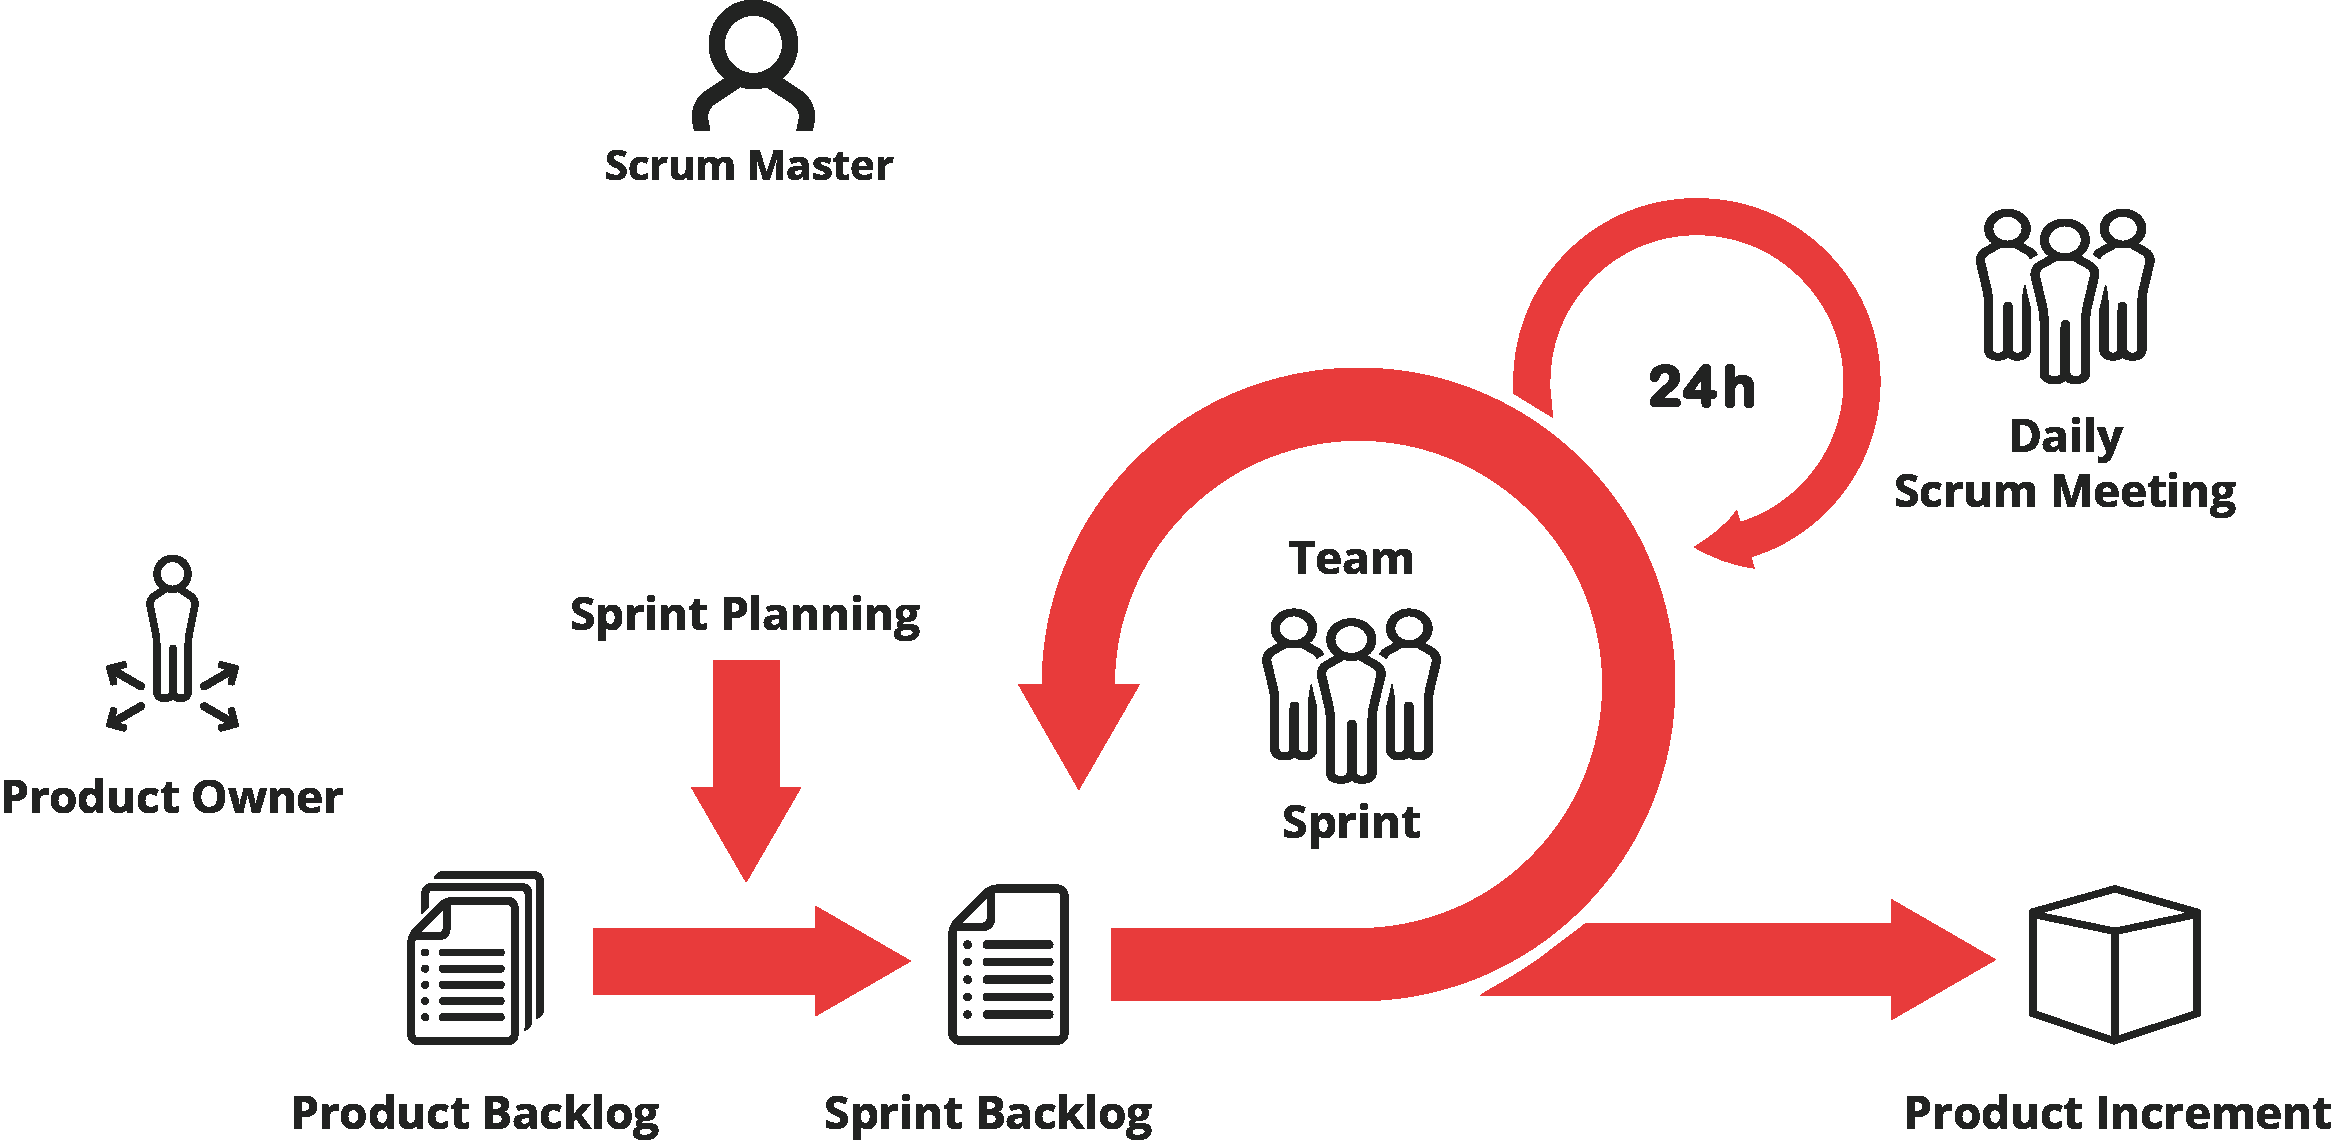
\includegraphics[width=0.7\textwidth]{pictures/scrum}
 \caption[Agiles arbeiten mit Scrum]{Agiles arbeiten mit Scrum \cite{scrum2018}}
 \label{fig:scrum}
\end{figure}

Die Verantwortlichkeiten liegt beim sogenannten Scrum-Team, welches sich aus folgenden Rollen ergibt:

\begin{center}
	\begin{tabular}{ ccc }
	\toprule
	  {MB-Adresse (dec)} &
	  \multicolumn{1}{c}{MB-Adresse (hex)} &
	  \multicolumn{1}{c}{Beschreibung}\\
	
	\midrule
	00000\dots31999 & 0x0000\dots 0x7CFF & FC1/FC2 \\
	32000\dots63999 & 0x7D00\dots 0xF9FF & FC3/FC4/FC6/FC16/FC23/FC66 \\
	00000\dots31999 & 0x0000\dots 0x7CFF & FC3/FC6/FC23/FC66 \\
	32000\dots63999 & 0x7D00\dots 0xF9FF & FC1/FC2/FC5/FC15 \\
	\bottomrule
	\end{tabular}
	\captionof{table}{Verteilung der abgeänderten Scrum-Rollen} \label{tab:scrumrollen} 
\end{center}


\ldots


\section{Systemkonzept und theoretische Realisierung} \label{Systemkonzept und theoretische Realisierung}

\ldots


\section{Projektmanagement} \label{Projektmanagement}
\subsection{Zeitplanung} \label{Zeitplanung}

\ldots



\subsection{Kostenaufstellung} \label{Kostenaufstellung}

\ldots

\subsection{Projektplanung} \label{Projektplanung}


